\chapter{関連技術}
\label{chap:related_works}

本章では,本研究における手法を選ぶに当たって,既存の基盤手法の比較と,基盤技術として使用するRDMA(Remote Direct Memory Address)に関して述べる.

\section{オペレーティングシステム解析手段}

本セクションでは,\ref{chap:introduction}で述べた,既存のオペレーティングシステムおよびプロセスの解析技術について述べる.
コアダンプを用いた静的解析や,kgdb,VMを用いた解析に関して述べた後,その手法の一つであるlibvmiについて述べる.

\subsection{コアダンプを用いた静的解析}
\label{subsubsection:core_dump}

コアダンプとは,カーネルクラッシュダンプとも呼称する\cite{dump}が,
この技術は,オペレーティングシステムが何かしらの原因でパニックに陥った際に,停止した時点のメモリの情報を2次記憶装置に書き出し,あとで解析できるようにするための機構である.

Linuxにおいては,\verb|kdump|と呼ばれる機構を通して,メモリダンプを取得する.
適切に設定をしておくことで,システムはパニックに陥ったのち,\verb|kdump|を実行するためだけの緊急用のカーネルを起動し,メモリの内容を書き出していく.

ここで得られたファイルを,Volatility\cite{Volatility}のようなツールを用いて,オペレーティングシステムが停止する前にどのような状態にあったのかに関する解析を行う.

\subsubsection{Volatility}
\label{subsubsection:Volatility}

Volatility\cite{Volatility}とは,\ref{subsubsection:core_dump}などを用いて取得した静的なメモリダンプに対して,解析を行うソフトウェアである.

Volatilityでは,取得したメモリダンプがアトミックである前提のもと,オペレーティングシステムがどのような状態にあったかを解析するためのものである.
Volatilityで使用されている手法は本研究において大いに参考になるが,このソフトウェアは,静的なファイルにのみ対応している.
つまり,動作中のコンピュータに対する解析を行うことはできない.

\subsection{VMを用いた解析}

VMを用いた解析では,監視したいホストをVMとして起動することで監視を実現する手法である.

VMとして起動する際に用いる技術としては,QEMU\cite{qemu}がある.qemuとはコンピュータ全体をエミュレーションし,仮想マシンとしてオペレーティングシステムを起動するためのソフトウェアである.
qemuではプロセッサだけでなく,マウスやキーボードなどの周辺機器をエミュレートするため単体での使用も可能だが,
近年では,Linuxカーネルに実装されている仮想化モジュールであるKVM\cite{kvm}と組み合わせて使用することも多くなった.

この手法では,\ref{fig:vm_arch}に示したように,ホストOSの上でqemuを通してゲストOSを実行する.

% \begin{figure}[htbp]
%     \caption{監視対象ホストをVMとして起動する場合}
%     \label{fig:vm_arch}
%     \begin{center}
%         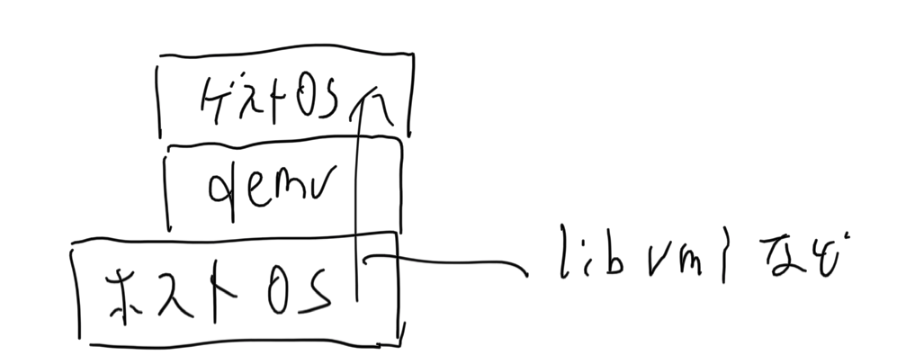
\includegraphics[bb=0 0 1000 340,width=15cm]{img/tegaki/01_vm.png}
%     \end{center}
% \end{figure}

\subsubsection{libvmi}

QEMUの上で実行するlibvmi\cite{osti_1334968}というものがあり.これを使用した解析も可能である.

詳しく書く

\section{RDMA}

RDMA(Remote Direct Memory Address)とは,DMA(Direct Memory Access)\cite{amini1995system}転送をネットワーク越しに行う技術のことである.
DMAは,メモリを読まれる対象のホストのマザーボード上のPCIeBusの上で動作する規格であるため,メモリを読まれる対象のホストのCPUコアを介さない通信が可能である.
RDMAでは,ネットワーク越しにDMA messageを発行する技術であり,解析の際にCPUコアのリソースを使用しない,ゼロ・オーバーヘッド動作環境を実現することができる.
さらに,監視対象ホストのオペレーティングシステムの状態に依存しない,つまり,電源さえ入っている状態であれば,動作中であろうとカーネルパニックが発生している状態であろうと,
DMA messageを発行し,結果を得ることが可能となる.

% \begin{figure}[htbp]
%     \caption{PCI Express}
%     \label{fig:zentai}
%     \begin{center}
%         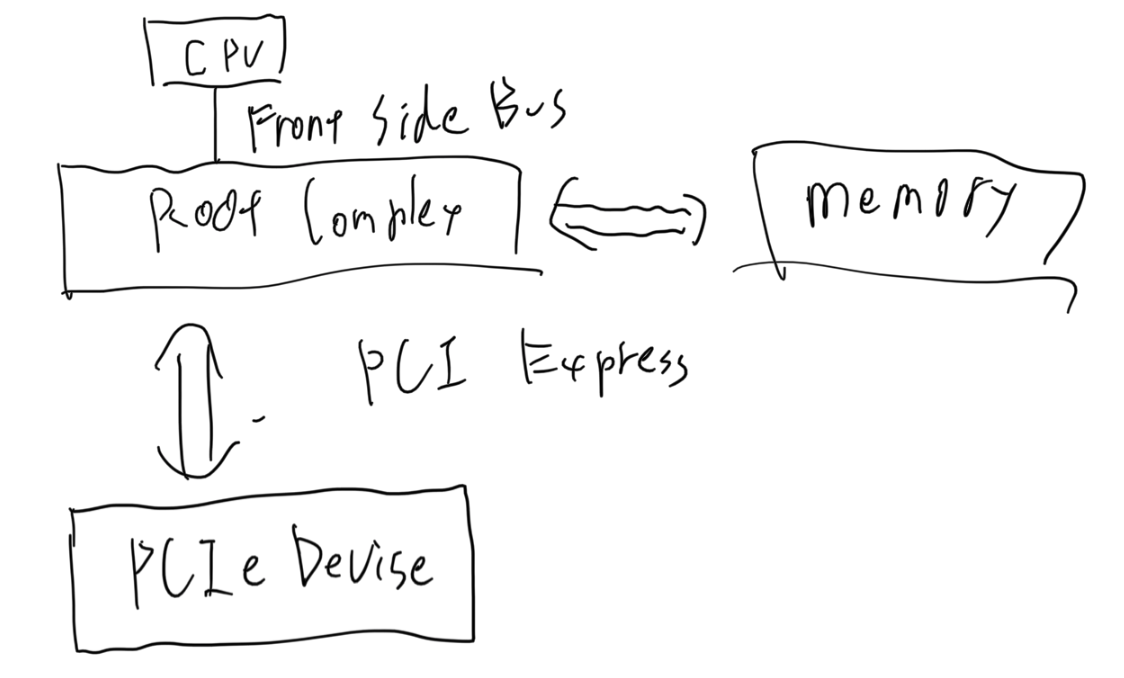
\includegraphics[bb=0 0 1000 400,width=15cm]{img/tegaki/pcie.png}
%     \end{center}
% \end{figure}

\subsection{InfinibandにおけるRDMA実装}

制約がかなり厳しく,本研究の用途には適さないということを書く

RDMAの実装として,Infiniband\cite{islam2012high}におけるRDMA実装がある.

しかし,infinibandにおけるRDMA\cite{infiniband-rdma}では,実際のパケットの送受信を行うのは,Host Channel Adapter(HCA)であるが,このHCAがアクセスできる領域はあらかじめMemory Regionとして監視対象ホストのOSにされている.
アクセスできる領域の仮想アドレスと物理アドレスの変換表はHCAが保持し,変換した上でアクセスする.
そのため,infiniband RDMAでは規格上,許可された仮想アドレス空間の指定しかできず,メモリ空間の全てを参照することはできない.
したがって,infiniband RDMAでは,オペレーティングシステム全体の監視・解析を行うことは難しい.
